 \documentclass[a4paper,twoside]{article}

\usepackage{epsfig}
\usepackage{subfigure}
\usepackage{calc}
\usepackage{amssymb}
\usepackage{amstext}
\usepackage{amsmath}
%\usepackage{amsthm} --commented by martin 22nov2013.
\usepackage{multicol}
\usepackage{pslatex}
\usepackage{apalike}
\usepackage{SCITEPRESS}
\usepackage[small]{caption}

\subfigtopskip=0pt
\subfigcapskip=0pt
\subfigbottomskip=0pt



%%%%%%%%%%%%%%%%%%%%%%%%%%%%%%%%%%%%%%%%%%%%%%%%%%%%%%%%%%%%%%%%%%%%
%% Packages not belonging to the original style of the conference %%
%%%%%%%%%%%%%%%%%%%%%%%%%%%%%%%%%%%%%%%%%%%%%%%%%%%%%%%%%%%%%%%%%%%%

\usepackage[usenames,dvipsnames]{xcolor}
\usepackage{listings}
%\usepackage[thmmarks]{ntheorem}
\usepackage[thmmarks,amsmath]{ntheorem}

\newcounter{numberInTrivlist}

\newenvironment{numtrivlist}{\begin{list}{\rm \arabic{numberInTrivlist})} 
                                         {\usecounter{numberInTrivlist}
                                          \setlength{\leftmargin}{0pt}
                                          \setlength{\rightmargin}{0pt}
                                          \setlength{\itemindent}{12pt}
                                          \setlength{\listparindent}{0pt}}}
                            {\end{list}}
                            
\lstset{numbers=right, numbersep=5pt, numberstyle=\tiny, stepnumber=1,escapechar=\!,columns=fullflexible,
        morekeywords={procedure,let,for,do,if,then,else,add,choose,end,while,true,false,rise,exception,extend,resume,to}}

\newcommand{\openbox}{\leavevmode
  \hbox to.77778em{%
  \hfil\vrule
  \vbox to.675em{\hrule width.6em\vfil\hrule}%
  \vrule\hfil}}

\theoremstyle{plain}
\theoremheaderfont{\normalfont\bfseries}
\theorembodyfont{\normalfont}
\theoremseparator{}
\theoremindent0cm
\theoremnumbering{arabic}
\newtheorem{algo}{Algorithm}

\theoremstyle{plain}
%\theoremheaderfont{\normalfont\itshape}
\theoremheaderfont{\normalfont\bfseries}
\theorembodyfont{\normalfont}
\theoremseparator{}
\theoremindent0cm
\theoremnumbering{arabic}
\theoremsymbol{\ensuremath{\openbox}} 
\newtheorem{example}{Example}


\theoremstyle{plain}
\theoremheaderfont{\normalfont\bfseries}
\theorembodyfont{\normalfont}
\theoremseparator{.}
\theoremindent0cm
\theoremnumbering{arabic}
\theoremsymbol{\ensuremath{\Box}} 
\newtheorem{defi}{Definition}

\theoremstyle{plain} 
\theoremsymbol{\ensuremath{\Box}} 
\theoremseparator{.} 
\newtheorem{prop}{Property}







\begin{document}

%\title{Authors' Instructions  \subtitle{Preparation of Camera-Ready Contributions to SCITEPRESS Proceedings} }

\title{SLA guided data integration on cloud environments 
       \subtitle{Brokering energy for providing sustainable consumption} 
       }

%\author{\authorname{First Author Name\sup{1}, Second Author Name\sup{1} and Third Author Name\sup{2}}
%\affiliation{\sup{1}Institute of Problem Solving, XYZ University, My Street, MyTown, MyCountry}
%\affiliation{\sup{2}Department of Computing, Main University, MySecondTown, MyCountry}
%\email{\{f\_author, s\_author\}@ips.xyz.edu, t\_author@dc.mu.edu}
%}

\keywords{The paper must have at least one keyword. The text must be set to 9-point font size and without the use of bold or italic font style. For more than one keyword, please use a comma as a separator. Keywords must be titlecased.}

\abstract{
This paper proposes data integration  (lookup, aggregation, correlation) strategies adapted to the vision of the economic model of the cloud such as accepting partial results delivered on demand or under predefined subscription models that can affect the quality of the results; accepting specific data duplication that can respect privacy but ensure data availability; accepting to launch a task that contributes to an integration on a first cloud whose SLA verifies security requirement rather that a more powerful cloud but with less security guarantees in the SLA. 
}


\onecolumn \maketitle \normalsize \vfill

%%%%TO BE DELETED BEFORE SUBMITTING%%%%%%
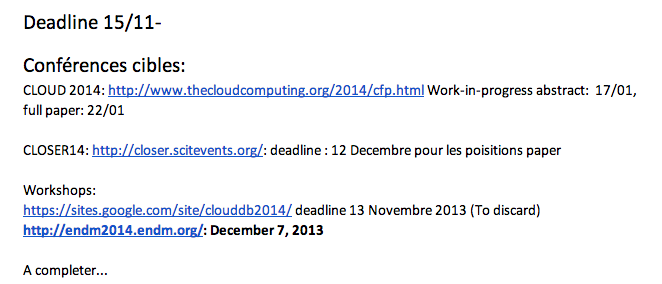
\includegraphics[width=0.5\textwidth]{figs/plan.png}



\section{\uppercase{Introduction}}
\label{sec:introduction}
%\color{red}
%


\color{black}
The advent of cloud computing imposed a new model for resource consuming that is not concerned
 with resource availability but with the \textit{technical and economic} conditions to be fulfilled in order to access a potentially unlimited resources. Integrating and processing heterogeneous data collections, calls for efficient methods for correlating, associating, filtering them taking into consideration their "structural" characteristics (due to the different data models) but also their quality, e.g., trust, freshness, provenance, partial or total consistency. 
Existing data integration techniques have to be revisited considering weakly curated and modeled data sets. This can be done according to quality of service (QoS) requirements expressed by their consumers and Service Level Agreement (SLA) contracts exported by the cloud providers that host  these collections and deliver resources for executing the associated management processes.
In fact,  the interest of SLA has been demonstrated  in data analysis but has not been yet widely considered for integrating data. Therefore, we believe in the benefits of SLA-based data integration as an approach for better meeting  user requirements.
\color{red}
In order to do so, several granularities of SLA must be considered: (i) at the cloud level: the SLA ensured by providers regarding data; (ii) at the service level, as unit for accessing and processing data, to be sure to fit particular service needs; and finally (iii) at the integration level i.e the possibility to process, correlate and integrate big data collections distributed across different cloud storage supports, providing different quality properties to data (trust, privacy, reliability, etc).


\color{black}
%To better understand our problem, let us consider an example from the domain of energy
%management. We assume we are interested in queries like: \textit{Give a list of energy providers that can provision 1000 KW-h, in the next 10 seconds, that are close to my city, with a cost of 0,50 Euro/KW-h and that are labelled as green?} \\
% The user demanded to apply a special encryption algorithm to sensitive data if data has to be transferred between providers or between physical sites during the integration process (Constraint1). Furthermore, the data providers could wish also that in case of a common use of their data within  an integration process, that this should be done assigning the less important privileges to the user w.r.t her credentials to access the different data (Constraint 2). We consider a simplified SLA cloud contract inspired in the cheapest contract provided by Azure: \textit{cost of \$0,05 cents per call,  8~GB of I/O volume/month, free data transfer cost within the same region,  1~GB of storage.} 
%The user is ready to pay a maximum of \textit{\$5 as total query cost}; she requests that only  \textit{green} energy providers should be  listed (provenance), with at least  \textit{85$\%$} of precision of provided data, even if they are not fresh; she requires an availability rate of at least 90$\%$ and a response time of  \textit{0,01 s}. She demands to contact only data providers with a threshold of trust . 

To better understand our problem, consider a massive open online course system (MOOC) where users produce and consume content according to the geographic area and expertise of participants. 
Producers are characterized according to their location, the type and topic of the content that they can provide, the access conditions (e.g. cost, inscription, or exchange unit), and the time window in which they can produce contents. 
Consumers are described by their location, their interests requirements during a certain interval of time, the maximum total cost they are ready to pay, or the resources they are ready to provide in order to get the service, and QoS requirements such as availability and how critical it is to consume a given type of content. 
The MOOC  aims at being privacy respectful of the students participating in courses.
 Providers  and consumers can ask to minimize the transfer of personal data  when they share/consume content.  According to the level of trust associated to data providers, the MOOC can use privacy preserving technics to let users share content anonymously  (Constraint1). Furthermore,  data providers could  also wish to give restricted data access credentials w.r.t. to their own, when their data are used  within  an integration process (Constraint 2).  
 
 %that this should be done assigning the less important privileges to the user w.r.t her credentials to access the different data 


  From this scenario we identify a set of issues that have to be addressed. First, how can the user efficiently obtain  results for her queries such that they meet her QoS requirements while respecting her subscribed contracts with the involved cloud provider(s)?  The user knows the low-level clauses of her SLA contract but she does not have an idea about the resources required to satisfy her requirements (SLA exported by services, example of Constraint 1).  Second, data services contracts should not be neglected in an integration process (Constraint 2).   As data services are deployed in a multi-cloud context, there is a need to establish the rules on how integration can be made and in which conditions. In fact, integration could be sometimes realized enforcing all specified conditions; we can also expect situations where they can be verified partially. In any case, how should the results of  such a  complex process  be capitalized for further integration requests?
  
 In this paper, we present  a preliminary solution addressing the issues described above.  Our solution is SLA-guided: We assume that data services publish Agreed-SLA that describe their  static and dynamic QoS measures in specific registries.  Thanks to an extended query rewriting process, a new kind of SLA is derived to match user preferences with low level agreed SLAs exported by services. The derived SLA allows to choose  services (w.r.t user demands) that can contributed for answering a query. Once data services have been chosen, the integration process will be guided by an integration SLA, negotiated taking into account user requirements and inter-cloud contracts.
%  Particularly, for queries that call several services deployed  on different clouds. 
%  Among them first,Furthermore, for a non specialist user, she do not realize what is the level of ressources she need to apply the encryption level asked  for. 
%  As data services are deployed in a multi-cloud context, there is a need to establish the rules on how integration can be made. 
%  concerns the context in which data will be used among clouds when data services are deployed in a multi-cloud configuration. How can the specified services requirements be enforced? And finally, data integration in this context faces an heterogeneity problem at different levels but specially in the scenario we are interested in, in data deployment conditions, the SLA expression language, the level security is taken into account in SLA contract.

 
 \color{red}
Accordingly, the remainder of this paper is organized as follows. Section \ref{sec:relWork} presents related works that address SLA modelling, integration and SLA guided data management processes. Section \ref{sec:incremental} gives an overview of our approach for integrating data sets provided by services (i.e., DaaS) by conciliating SLA's provided by services and user's profiles expressing QoS preferences. Profiles specify preferences about the data they want to consume and the conditions in which they must be processed and delivered. 
%Section \ref{sec:useCase} presents a use case for illustrating the interest and use of our approach. 
Finally \ref{sec:conclusions} concludes the papers and discusses future work.

\color{black}

\section{\uppercase{Related Work}}
\label{sec:relWork}

%\begin{itemize}
%\item Cloud computing represents a novel on-demand computing approach where resources are provided in compliance to a set of predefined non-functional properties specified and negotiated by means of Service Level Agreements (SLAs).  SLA currently exploited in the cloud allows service providers and cloud client to fix the resource level that should be used either by a service for the service provider or by the client in the case of service invokation. SLA could concern all types of the services on the cloud (IAAS, PAAS or SAAS). One of the weakness of SLA for the client is that they express low level clauses like storage amount use or virtualization level. In fact when a client launches a task on the cloud, she has unlikely Q \& S requirement rather than low level features. Recently we notice the existing of a lot of works with the objective to fill the gap.  Emeakaroha and al propose in \cite{5547150}  a cloud component that acts autonomously based on low level  monitored features after analysing them towards high level clauses expressed by the user. Moreover, another difficulty to enforce an SLA is to measure and identify, starting from a high level SLA clause, how could it be declined at different layers in the cloud. Therefore in \cite{Dastjerdi:2012:DOA:2275356.2275360} the authors describe a semanticSLA which can be understood by all parties including providers,
%requestors, and monitoring services. One of the major objectives in the cloud is to anticipate SLA violation and to assess SLA failure cascading on violation detection. \cite{Dastjerdi:2012:DOA:2275356.2275360} proposes an SLA dependency modeling using Web Service Modeling Ontology (WSMO) to build a knowledge database.  \cite{5547150} proposes to anticipate failure by analysing the monitored feature and to act by anticipation. in \cite{5614035}, the authors propose LAYSI, a layered solution that minimizes user interactions with the system and prevents violations of agreed SLAs. 
%On the other hand SLA contracts do not cover all client requirement. There is still a lack in some domain.....(to be completed)

%\item some 

The advent of cloud computing imposed a new model for resource consuming that is not concerned
 with resource availability but with the \textit{technical and economic} conditions to be fulfilled in order to access a potentially infinite set of resources. 
Service Level Agreements (SLA)~\cite{SLA} can be used in the context of cloud computing to establish those conditions. The adoption of SLAs relies on two principles: (i) The negotiation of conditions in which services will be provided and that are statically agreed between the parts and (ii) The monitoring of these conditions during the use of cloud resources in order to detect SLA contract violation.

%The agreed conditions should be explicit and quantifiable.
%They should be part of the contract between the client and the service provider.
%Their quantifiable nature makes it possible for the conditions to appear as non-functional requirement to be imposed to each individual service.
%SLA could concern all types of services on the cloud (IaaS, PaaS or SaaS).

%SLA compliance may be ensured by construction or may be monitored during the execution of the service.
%Monitoring SLAs is normally part of the infrastructure provided by the cloud.
%Service monitoring may incur in extra processing costs.

%SLA currently exploited in the cloud allows service providers and cloud clients to describe the amount of resources to be simultaneously used and also the conditions to use them.
%This limit may apply both for the service provider and the client (in the case of service invocation). 

%Negotiating a SLA may be a difficult task.
%Indeed, 
SLAs are normally expressed in terms of \textit{technical}, quantifiable measures, like the storage space size  or the degree of virtualization. 
On the user side, the interest is normally on \textit{service} delivery measures such as QoS requirements.
The challenge is to couple technical and service delivery measures expressed in SLA in order to agree on the conditions in which they will interact. Existing works use matching and negociation techniques for addressing this challenge.  
For instance,~\cite{5547150} 
proposes a bottom-up approach based on a cloud component that monitors technical measures, analyses and matches them to service delivery (high level) clauses expressed by the user.
  \cite{Dastjerdi:2012:DOA:2275356.2275360} describes a \textit{Semantic SLA} that can be understood by all parties including providers, consumers, and monitoring services.
Their goal is, starting from a high level SLA, to measure and identify how to derive SLA measures  at different layers of the cloud.  \cite{Ortiz:2013:VPS:2486767.2486772}
  proposes a set of templates to  cloud data services users, each specifying the query type that can be executed with some tread-off in time and corresponding cost.  The client  chooses among the proposed tempates the one that best corresponds   to her requirements. \cite{6141307} proposes a set of matching algorithms to identify compatible cloud providers for a given requirements specification by matching SLA parameters. Cloud SLA parameters and application requirements are represented by two models using RDF. RDF definitions are then converted into graph representations. An Induced Propagation Graph is calculated using both models to establish a correspondence between them.


%{\color{red}
%One of the major objectives in the cloud is to anticipate SLA violation and to assess SLA failure cascading on violation detection. 
%\cite{Dastjerdi:2012:DOA:2275356.2275360} proposes an SLA dependency modeling using Web Service Modeling Ontology (WSMO) to build a knowledge database.  
%\cite{5547150} proposes to anticipate failure by analysing the monitored feature and to act by anticipation. 
%In \cite{5614035}, the authors propose LAYSI, a layered solution that minimizes user interactions with the system and prevents violations of agreed SLAs. 
%}

Recent  works on SLA are devoted to extend  SLA for including  security concerns. 
\cite{6274042} propose an extension of the WSAgreement, initially developed by the GRAAP
working group. 
Security constraints are expressed over the service description
terms (SDTs) and the service level objectives (SLOs) of the SLA. 
This leads to an interoperable security expression that can be used by users for comparing security levels of different cloud service providers. 
\cite{LunaGarcia:2012:BCS:2381913.2381932} focuses on how to build a SEcSLA Template starting from gathering then categorizing a set of security statements using a semantic tool. 
The designed template is then used both to express user security requirements and cloud service provider security provision.
Finally, some works  deal with SLA violation anticipation and SLA failure cascading on violation detection.  \cite{Dastjerdi:2012:DOA:2275356.2275360}  proposes an SLA dependency model using Web Service Modeling Ontology (WSMO) to build a knowledge database. \cite{5614035} proposes to anticipate failure by analysing the monitored feature. 
\cite{5614035} proposes LAYSI, a layered solution that minimizes user interactions with the system and prevents violations of agreed SLAs.

%=====================================

%Another issue in the SLA management domain is how to let cloud service provider offer fit the best user requirements. In fact, current SLA are only resource oriented and lacks in expressing client requirement in service quality and characteristics. Plenty of works tends to fill the gap. First by proposing predefined templates;. 

  
%  In \cite{LunaGarcia:2012:BCS:2381913.2381932,}, the authors propose to do a mapping of both user SecSLA requirements and CSP SecSLA provisions on a set of Quantitative Policy Tree(QPT), where atomic capabilities are mapped on leaves and intermediate represents coarse provisions with some logical operators (AND, OR). The mapping allows to give a quantitative benchmarking to each CSP offer with respect to user requirements that lets the user be able to make a choice. For more experienced users, \cite{6313668} proposes an extensible specification grammar that allows to express user and application-specific requirements in using a cloud data service. This allows to customize the SLA management at the cloud side. Emeakaroha and al propose in \cite{5547150}  a cloud component that acts autonomously based on low level monitored features after analysing them towards high level clauses expressed by the user. Moreover, another difficulty to enforce an SLA is to measure and identify, starting from a high level SLA clause, how could it be declined at different layers in the cloud. Therefore in  \cite{Dastjerdi:2012:DOA:2275356.2275360}  the authors describe a semantic- SLA which can be understood by all parties including providers,requestors, and monitoring services. 
% \cite{6141307} proposes a batterie of matching algorithms to identify compatible cloud provider for a given requirements by matching SLA parameters.
%In this work, SLA parameters of the cloud are defined in a cloud capable model and application's requirements are defined
%in an application requirement model. Those models specified firstly using RDF, are converted into graph structures using Jena APIs.
%From those graphs a Pairwise Connectivity Graph is defined and an Induced Propagation Graph is calculated.
%Pairwise Connectivity Graph is constituted by nodes called mappairs established when source and target nodes from initial graphs have the same property edge.
%For the Propagation Graph each edge is given a weight. Finally, a Similarity propagation graph is constructed based on an initial mapping between the RDF models, where mapping nodes are compared (subclass, superclass, equivalence relation) and the mapping is used in a similarity flooding algorithm which is filtered out to only the instance node pairs that have similarity value greater than zero.
%  



 
 % \item data integration (cf. travaux Gonzalez) 
%\end{itemize}


%\section{\uppercase{SLA based data integration}}
%\label{sec:slaDataInteg}
%{\color{green}
Overview of our approach that will include:
- An SLA Model: including security issues

- A multi cloud environment representation

- On demand incremental data integration strategies
}

\begin{figure*}
\caption{General architecture of an SLA guided  data integration system.\label{fig:arch}}
\end{figure*}

Figure~\ref{fig:arch} shows the general architecture of an SLA guided data integration system that is supported by data services which are data providers deployed in a cloud and that provide agreed SLA’s. 
These descriptions are stored in a directory together with meta-data about the way queries are evaluated for producing results. 
The system uses this information  by query processing and monitoring modules for rewriting queries according to given quality of service (QoS) preferences expressed by a data consumer, for example a user.

\subsection{SLA model}
\label{sec:slaModel}

\begin{itemize}
\item Expression haut niveau du SLA en termes de préférences qui doit converger avec le SLA technique des services.
  \begin{itemize}
  \item (Souhait de temps de réponse, coût des services, espace de stockage,  
  \item Templates pour exprimer le SLA
  \item Intégration: modèle pivot de SLA
\end{itemize}

\item SLA violation contrôlée avec des mechanisms de monitoring.
\item Que ce que devient l’intégration de données par rapport au SLA
\item Création dynamique de SLA → niche de marché: étant donnée deux SLA fabriquer un SLA d’intégration
\end{itemize}


In order to propose an SLA guided continuous data provision and integration, we need to think about possible steps from the request to the delivery of the result sets. Indeed, let consider a request R launched by a user who specifies a number of constraints on the environment execution. Executing this query requires first a semantic analysis which will subdivide R into a set of sub-queries, in such a way that each sub-query can be processed by a DataService deployed on the cloud. One may think to a first filter to remove the individual services which do not meet some or all of the constraints expressed by the user. This first stage can be defined as a vertical mapping SLAs given the high level SLA described by the user (i.e. macroscopic constraints: execution time, pay / no pay, data reliability, data source). The system should be able to find relevant service compositions that respond to the query and, when combined, meet the constraints imposed by the user (High level SLA).
To meet this objective, it is necessary to compare the SLA services to combine, in order to check if their joint use is compatible with the individual SLA. This step may lead either to the rejection of integration in case of total incompatibility, or to a negotiation between SLA which will lead us to the proposal for a negotiated SLA integration and thus the need for an adaptive Template.
The negotiation of this type of SLA depends strongly on the request sent and the services deployed at the arrival time of the application on the cloud. This negotiation can be expensive and may not scale well. It is therefore crucial to provide proactive mechanisms for optimizing the production of such SLA. We believe that the optimization of this process can occur at two levels, firstly at the level of SLA previously traded, and secondly at the level of partial or total results. Indeed, queries requesting the same services compositions will have clauses in their SLAs that are more conditions of use of the infrastructure (ie not touching the data). For two different queries, they will be negotiated in the same way. These previously negotiated SLAs are reusable.
In a second time, we think optimizing this process on the data storage mechanisms to cache intermediate results, individually or in partial or complete combination depending on the terms of SLA services (data access, intermediate storage capacity , cost of storage , etc ... ).
Given this proposal, we identify several issues:
- Level modeling would require a model that allows the representation of SLA integration.
- There should also be a template for representing the requirements expressed by the user
- A mining component to identify, from the requirements expressed in the template by the user, and before the analysis of the application, the candidate integration SLA to use or adapt according to the request. This implies mapping between property and expressed clauses being.

\subsection{Query Rewriting}
\label{sec:queryRew}

{\color{red}
Here Martin will explain the rewriting problem.
}

\subsection{Data and query models}
\label{sec:dqm}

TBD.


\section{\uppercase{SLA based incremental data integration}}
\label{sec:incremental}
To answer the needs expressed above, we propose an SLA guided, security-aware continuous data provision and integration approach performed within a multi-cloud service oriented environment  (see
%starting from the processing of the query  to the delivery of the results.
Figure~\ref{fig:arch}). In this section, we present  step-by-step data integration process with the implied  SLA categories.

In our context, data are exposed as  a set of data services on different clouds. In our example of MOOC system presented above, several producers will supply equivalent content for a given period of time  that will be chosen with respect to the  preferences expressed by a consumer. 

Given a query $Q_1$ expressed as Datalog-like program or an SQL-like expression, including spatio-temporal attributes and preferences.
For instance, the following query ``\textit{List of English poetry content providers that can provide commented Emily Dickinson poems that are close to my city and that are labelled as experts, where the total cost is not higher to 1 dollar, with using only services that preserve her anonymity}''. 

The abstract Inter-Cloud Layer (ICL) is in charge of delivering a result to the received query. ICL will first identify a set of semantic functionalities that fit the  query and associated services, stored in the service description registry.

Assume that there are four content providers on English poetry that can be queried individually and two hubs that collect information from other sources like social network groups and hash tags.
Hubs will store content about given topics on  English poetry, available from particular producers (e.g., participants of a given course).
We represent these services by { e$_1$, \dots, e$_4$} and {h$_1$} and {h$_2$}. We suppose that hubs will have the same interface as individual service providers.
We also suppose the existence of two free location services exporting the following interface: {loc(IP) $\rightarrow$ $\langle$ X, Y$\rangle$}, meaning that given an IP address it returns a geographic position expressed as a pair of coordinates. 
All these services can potentially be combined for answering queries.


%shows the general architecture of an SLA guided data integration system. 
%It accesses data services which are data providers deployed in a cloud  that provide agreed SLA's. 
%The whole process is monitored to determine whether a computed SLA is being honoured while a query is evaluated. 

%These descriptions are stored in a directory together with meta-data about the way queries are evaluated for producing results. 
%The system uses this information  by query processing and monitoring modules for rewriting queries according to given quality of service (QoS) preferences expressed by a data consumer, for example a user.The following lines describe how this query is evaluated according to our approach. 

\begin{figure*}
\center{
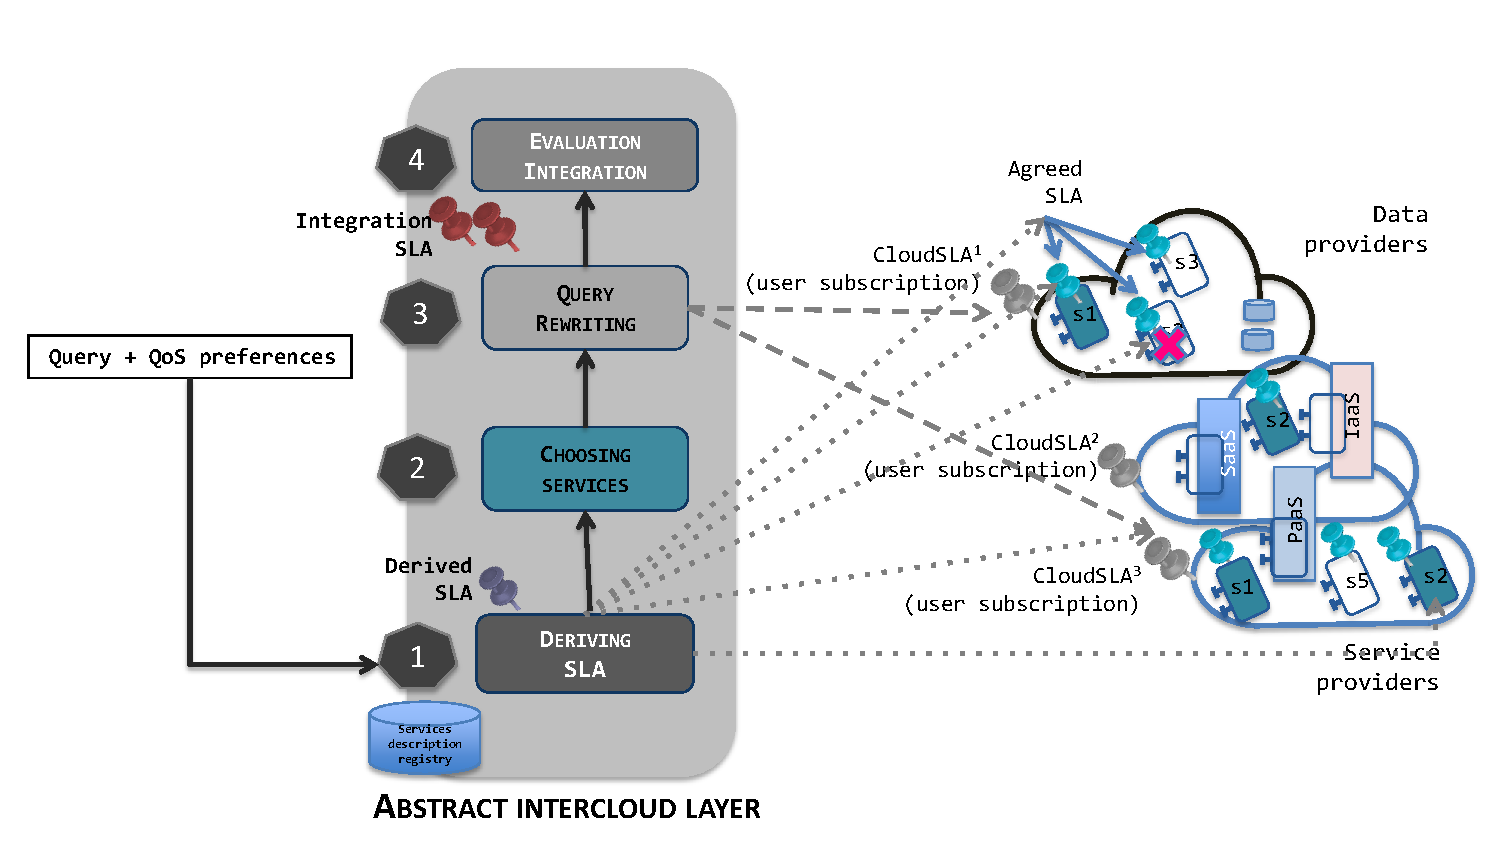
\includegraphics[width=0.75\textwidth]{workflow.pdf}
\caption{Phases of an SLA guided  data integration workflow.\label{fig:arch}}}
\end{figure*}

%In order to illustrate our approach, consider a massive open online course system (MOOC) that aims at being privacy respectful of the students participating in courses and produce and consume content according to the geographic area and expertise of participants. 
%Producers are characterized according to their location, the type and topic of the content that they can provide, the access conditions (e.g. cost, inscription, or exchange unit), and the time window in which they can produce contents. 
%Consumers are described by their location, their interests requirements during a certain interval of time, the maximum total cost they are ready to pay, or the resources they are ready to provide in order to get the service, and quality of service requirements such as availability and how critical it is to consume a given type of content. 
%An energy exchange market is established in order to continuously trade  content provision/consumption ensuring that all consumers will have the content they require at every moment.

Each deployed service exposes an \textit{agreed SLA} that specifies the economic cost per call, the maximum number of calls that can be done per day, the availability of the service, the average response time when a method is called, the reliability, the privacy of the produced data (whether they can be stored or not), the precision, freshness and provenance of the produced data, as defined below:

%NOTE: Agreed SLA are client-provider slas... --MARTIN

\begin{trivlist}\sf\footnotesize
\item[~-~agreedSLA$_i$:] $\langle$cost, availability, freshness, provenance, data access control, certified reputation level, location, duration$\rangle$. 
 \end{trivlist}
 
Some of these measures ({cost/call, maxCall/day}) are static and explicitly specified by the service provider. 
In contrast, the other measures should be computed by monitoring the conversations between the service and the applications that contact it.  It is the case for service reputation that will condition the way personal user data will be anonymized (Constraint1).  Some measures will be instantiated depending on the context of  the service invoked within a multi-cloud environment. It is the case for constraint 2 expressed above:   user data access credentials should be calculated according to the clouds hosting different data services.
An \textit{agreed SLA} is expressed through an  XML document using the specification WSLA (Web service level agreement \footnote{\footnotesize http://www.research.ibm.com/people/a/akeller/\-Data/WSLASpecV1-20030128.pdf}).

Examples of computed measures are the cost of retrieving the list of ``expert'' Emily Dickinson poems providers within a region with their cost. 
The cost is determined by the  cost of the calls. 
This request  includes the price of calling a service (e.g.,  between 0,25 - 0,50 euros depending on the data service), plus the price of data transmission according to the amount of transmitted MegaBytes through the network, the type of subscription of the user for using the network and also the cost of applying encryption algorithm if asked for. The second computed measure is service reputation that is calculated according to the feedback obtained when application contacts the service.




As aforementioned, an a-priori SLA enforcement mechanism is mandatory to assess data integration feasibility.
To this end, non-functional characteristics of the content provision services ({i.e e$_1$, ... e$_4$}) are calculated by specific cloud services (SCS) that enforce SLAs  and which should present an API, composed of a set of methods such as:

\color{green}
\begin{trivlist}\sf\footnotesize
\item[~-~]estim-cost$_i$(contents, req\_size, cost, prov\_size, loc), 
%QoS preferences$_\mathit{user}$, -- These should be in the query... not in the concrete services specification.
agreedSLA$_i$.

\item[~-~]engage$_i$(contents, req\_size, payment), agreedSLA$_i$.
\end{trivlist}

 

%Given user expressed QoS preferences ({QoS preferences}$_\mathit{user}$) and {agreedSLA}$_i$, 
The first method allows to obtain for each service $e_i$ the estimation of the budget (in our example, of a given course (content)) and a required minimum size. In other words, it will returns the cost of the data, as well as its actual size and location.
 
The second method is used to engage in a data service (in our example a course data service) and will be used later if the service is retained for a composition that answer the query.

 
%The user will ask for a given derived SLA to which the provider may agree.

ICL by asking SCS for each semantic functionality, obtain the set of potential services that satisfy both user preferences and  service offering described through their \textit{Agreed SLAs}. 
Indeed, the query $Q_1$ has two parts: the one that corresponds to the content asked for by the user  that will be solved by combining data services and the \textit{user preferences}, noted by {QoS preferences}$_\mathit{user}$:
\begin{trivlist}\sf\footnotesize
\item[~-~QoS preferences$_\mathit{user}$: ] $\langle$cost, freshness, provenance, location, duration, privacy-preserving$\rangle$. 
\end{trivlist}

\color{black}

Let us suppose that for this query the user is ready to pay a maximum of \$1 as total cost; she requests that content providers be certified as experts (provenance) even if their data are not fresh; she requires a contract duration of one week. Besides, she wishes her privacy be saved by adapting the anonymity process with regard to service reputation. The maximum total cost will condition also which kind of privacy preserving algorithms to apply.
 
\begin{trivlist}\sf\footnotesize
\item[~-~QoS preferences$_\mathit{user}$: ] $\langle$cost $\leq$ \$1, freshness = ``any'', provenance = ``certified'', location = ``close'', duration = 7 days, privacy-preserving=``reputation-based''$\rangle$. 
\end{trivlist}



Cloud providers also define their SLA contracts that specify the cost per request ({cost/request}), the volume of data that can be exchanged per month ({I/0 volume/month}), the cost of transferring data or applications within the same data center or between data centers ({datatransferCost/region}), the storage space ({storageSpace}). For example some cloud providers enable the customer to choose the zone to install PaaS services and deploy applications (e.g. zone 1 is Europe). If the customer wishes to deploy services in zone 1 but store data in zone 2 the transfer cost will change.

\begin{trivlist}\sf\footnotesize
 \item[~-~cloudSLA:]  $\langle$cost/request, I/0 volume/month, datatransferCost/region, storageSpace$\rangle$.
 \end{trivlist}
 
Illustration inspired in the lowest contract provided by Azure\footnote{Azure is a trademark of Microsoft Corporation.}: 
 \begin{trivlist}\sf\footnotesize
\item[~-~cloudSLA:]  $\langle$0,05 cents per call, 8 GB I/0 volume/month, free, 1 GB storage$\rangle$. 
\end{trivlist}


 
%A content request is expressed as a query that specifies contents about a given topic with QoS preferences, independently of the possible providers. 

   

\color{green}


The next step supervised by the ICL consists in elaborating a set of potential composition specifications via a query rewriting process:
Given the user query, specified as a sequence of abstract operations and the available services, specified in the same way, we use a Local-as-View approach~\cite{CostaAMR13} to obtain a combination of services that match the query specification.
The algorithm in~\cite{CostaAMR13} is being modified to deal with SLA and QoS user preferences.

\color{black}

In this paper, we are interested in rewritten queries that comply with the user preferences,  cloud SLAs and QoS preferences.
 This allows computing a result as follows: (i) User preferences (including cloud SLAs according to user subscriptions) and \textit{agreed SLAs} will be used to produce a \textit{derived SLA} to be associated to the query. These derived SLA will influence the choice of (data) services that will actually be used for building the result; (ii) Query rewriting for computing service compositions that can be used for  building query results. The \textit{agreed SLA} exposed by the chosen services is added as  conditions in  each re-written query expression; Two situations could arise: a full compliance of a composition with the \textit{derived SLA} or a partial compliance that requires a negotiation step. For both alternatives, an \textit{integration SLA} will be produced indicating the negotiation conditions and the implementation of the final integration; (iii) and Managing the integration process according to the \textit{integration SLA}.

 
%-----------------------------------------------------------------
\section{Derived SLA}
\label{sec:slaModel}
%-----------------------------------------------------------------

The key and original aspect of  our proposed data integration and provision process is  defined as a vertical mapping of user QoS preferences and agreed SLAs of potential com posable services. This  leads to a {\em derived SLA} that guides the evaluation of a query. 

%A query has associated preferences  expressed as macroscopic constraints (i.e. user preferences statement): execution time, pay / no pay, data reliability, provenance, freshness, privacy-preserving constraints, partial/full results, delivery mode. These constraints are coupled with the profile of the user which is in general stated in her cloud subscription (amount of assigned storage space, number of requests, I/O transfered Mega bytes, etc.). 

%As said before, we assume that services export their \textit{agreed SLAs} that define measures that can be either expressed as constants,  computed (dynamically) by monitoring the execution and conversations associated to services, and hybrid they can be statically stated  but they change at execution time.  A service  agreed SLA is expressed through an  XML document using the specification WSLA (Web service level agreement \footnote{\footnotesize http://www.research.ibm.com/people/a/akeller/\-Data/WSLASpecV1-20030128.pdf}). The service SLA measures  that we consider in our example are: cost, availability, freshness, provenance, location, duration of the engagement, privacy-preserving status. Other measures are associated to the conditions in which the service is called or to the precision and recall of their produced data given a request. 



Given agreed SLAs and a user preferences statement the challenge is to compute a  {\em derived SLA} that  maps SLA measures and preferences attributes.  
The derived SLA is defined as a set of measures that correspond to the user preferences computed as a function of different static, computed and hybrid measures. 
The derived SLA  will guide the way the query will be evaluated, and the way results will be computed and delivered.

In the example, some of the user preferences statement measures are used for defining a derived SLA that, as said in previous section, will guide the evaluation of the query. 
These measures are defined as a function of the measures used by the agreed SLAs and by the cloud SLA contract.
\begin{trivlist}\sf\footnotesize
 \item[~-~query total cost:] $\sum_{i = 1\dots n}$ cost(s$_i$) + data transfer + encryption cost $\leq$ \$1.
 \item[~-~availability:] {\em (of services involved)} $\geq$ {\sf 90$\%$}.
 \item[~-~freshness:] non.
 \item[~-~provenance:] all services involved must be $expert$.
 \item[~-~duration:] 7 days.
 \item[~-~I/0 volume/month:] 8GB.
 \item[~-~reputation level :] $\geq$ threshold.
 \item[~-~storageSpace:] 1GB.
 \end{trivlist} 
 
Therefore, we propose a classification of SLA measures that represents the combination of fine grained measures used by agreed SLAs and coarse grained measures used in user preferences statements. 
It specifies also how to compute coarse grained measures with fine grained ones. 
For example, data precision will be computed as a function of availability, freshness and provenance exported by data services. The derived SLA can be seen as a set of inequations that have to be solved during the execution of a service composition. Since some of them can only be determined at execution time, the decision on which services will participate in the evaluation of the query is approximated. We will discuss this issue in the next sections.

This step may lead either to the rejection of integration in case of total incompatibility, or to a negotiation between SLA which will lead us to the proposal for a negotiated SLA integration and thus the need for an adaptive setting.
Negotiation of this type of SLA depends strongly on the request sent and the services deployed at the arrival time of the application on the involved  clouds (i.e clouds holding services that satisfies user requests and that are candidate to service composition to answer the query). This negotiation can be expensive and may not scale well.
 
Given a query and its preferences statement, the system  finds  service compositions that produce results   meeting the required constraints, as discussed in the following section.

 
 
%-----------------------------------------------------------------
\section{Query Rewriting}
\label{sec:queryRew}
%-----------------------------------------------------------------

\color{red}
One point remain very crucial to fix: once the multi-cloud layer generate a list of derived SLA corresponding to Agreed-SLA of services that could match a part of the query, What should happen?  With whom rewritten query using user preferences is matched with SLA and which one (not clear in the paper.  This point should be discussed quickly. The workflow of SLA between the abstract layer and cloud is not so clearly described.

\color{green}
Answer by Martin: The agreedSLA will be included and merged with the SLA conditions obtained by the rewriting process. Only those compositions that comply with the agreedSLA will be presented as solutions to the user.
 
\color{black}
Query rewriting is a well-known problem in the database domain.
The problem consists in transforming an abstract query into a set (or list) of lower-level queries that can be solved by  available databases.
%Query rewriting is guided by the schema of  abstract and concrete databases.
%The answers to the lower level queries are combined in order to obtain the result to be returned to the user.
The query rewriting problem can be generalized to the case of services.
In this case, the query to be rewritten is seen as an abstract service composition, to be expressed in terms of concrete services.
Query rewriting techniques have been adapted to the context of service composition~\cite{BBM10,ZLC11,CostaAMR13}. 
In~\cite{CostaAMR13} the authors present an algorithm to automatically refine high-level specifications of service compositions into lower-level ones. 
The method is based on the MiniCon algorithm~\cite{PH01} for query rewriting.

The case of more general services (\textit{i.e}, services that maintain and update information) is a generalization of the information-provision case.
Unlike the simpler case, where only the service interfaces need to be considered, the general case requires considering the functional and non-functional aspects of the query and available services.
%In this context, the \textit{Local as View} (\textit{LAV}) methods of query rewriting~\cite{Levy2000} are suitable.
%In the LAV approach, 
The rewriting process is guided by the specification of both the query to be rewritten and the available services.
%The specification of the composition to be produced as well as the specification of each available service are used in the case of general services.
%These specifications may detail both the functional and non-functional behaviour of each service, including SLA.


We propose an approach that consists in generating translations of an abstract query into \textit{several}  compositions over concrete  services. 
%The solutions proposed are ranked and may be coded into concrete workflows as shown in the following section.  
The next example shows the main features of the approach proposed in~\cite{CostaAMR13} which is extended to the case of SLA-guided service-based data integration. 

%\begin{example}[Service Refinement by Rewriting]\label{Ex:rew1}
Let us consider the MOOC scenario, where people can participate on an content trading pool.
We suppose that this hypothetical MOOC has a large number of participants that sell their content  to  consumers. 
The MOOC has four information hubs, located in four different geographic locations, connected to other content providers.
Content providers may be  contacted directly, through the services of three different cloud providers.
Each cloud provider exports its own interfaces.
SLAs are defined for each individual content provider server and  each hub(agreed SLA)  , and also for each cloud provider (traditional SLA contracts). 

When an on-line consumer searches servers to buy/retrieve content, a composed web service is generated, in order to fetch each individual or hub service and to start  content retrieval procedures.
Depending on the location of the consumer and producers, different conditions and constraints may apply.
Also  cloud providers  publish the conditions for using their services.
These conditions and non-functional requirements (such as authentication or security requirements) should also been expressed in the user preferences and SLAs.

In this context, the user  expresses a content order, her location and payment information. A composite web service is  generated to fulfill the order.
The generated service composition should consider the nearest providers, in accordance to the agreed SLA.

In order to produce a personalized service composition for each user, the algorithm in~\cite{CostaAMR13} takes into account the specification of the composition (which may be produced by the user's browser, including context information).
The specification of each available service is also considered (this specification should be given by the service provider).
%~\hfill\openbox
%\end{example}

\color{green}
%Given a set of services that can possibly be composed and the derived SLA, a service composition must be produced.
%Some of the inequations of the derived SLA should be included in the service compositions that answers the query.

The agreedSLA will be included and merged with the SLA conditions obtained by the rewriting process. Only those compositions that comply with the agreedSLA will be presented as possible solutions to the user.
\color{black}

In the case of our query example the following composition can be used for answering it:

\begin{footnotesize}
\sf
\begin{tabbing}
 -~Q(myIPad\=dress, ``E.Dickinson'', 1MB, ``expert'', \$1, myCreditCard) $\equiv$ \\
 \>  myLoc = loc(myIPaddress), \\
 \>  estim$\_$cost(``E.Dickinson'', 1MB, cost, size, theirLocation), \\
 \>  query total cost + cost $\leq$ \$1,\\
 \>  availability $\geq$ 90$\%$, \\
 \>  freshness = any, \\
 \>  provenance = ``expert'', \\
 \>  duration = 7 days, \\
 \>  I/0 volume/month $\leq$ 8GB, \\
 \>  reputation level $\geq \lambda$ (the threshold) \\
 \>  storageSpace $\leq$ 1GB, \\
 \>  engage(``E.Dickinson'', size, myCreditCard).
 \end{tabbing} 
\end{footnotesize}

Our approach would generate a number $k$ of service compositions, combining as much as possible the services available such that the constraints of the derived SLA are verified. 
 Yet, the algorithm should be modified to take into account the different SLAs. The next example illustrates one of the limits of the automatic composition algorithm.

\color{red}
\begin{example}[Incremental queries]\label{Ex:rew2}
Let us return to the content  trade system of the MOOC example.
 Suppose that the user requires to retrieve a list of star providers  daily and weekly that can deliver ``\textit{5 Go}'' of expert content about Emily Dickinson poetry.
In this case, each individual and hub database will be queried and the list will be produced by adding data obtained from them, until the 5Go  capacity is reached.
Let us suppose that, in order to minimize the  communications between servers, the lists need to be produced incrementally.
In this case, the composition produced by the service refinement may need to include an iteration (to aggregate partial results). 
The data produced by the warehouse servers will be processed in batch and the process will end once the list reaches the desired capacity.

To our knowledge, the incremental production of a solution is beyond  the scope of the current methods for rewriting service compositions and represents a challenge to the area.
~\hfill\openbox
\end{example}

\color{black}

 
%-----------------------------------------------------------------
\section{Towards an integration SLA}
\label{sec:queryProcessOpt}
%-----------------------------------------------------------------
 Our data provision and integration approach relies on data services deployed on one or different clouds providers and it is delivered as a distributed DaaS on top of the clouds involved.  This DaaS  uses resources from a cloud and this use  is  guided by an economic model (stated in a cloud subscription) that puts a threshold on the amount of resources to be invested in a query evaluation process. It is thus important to optimize the use of these resources. 
   
The optimization of this process can occur at two levels: first at the level of agreed SLA exported by services.  Indeed, queries requesting the same services compositions will have clauses in their SLAs that are more conditions of use of the infrastructure (ie not storing the data produced by a service). Instead of recomputing the derived SLA every time, we propose to store it and reuse it for other queries. 
Second, pre-computed queries and partial results can be also stored in cache or in a persistent support. Rewriting results can be also stored and reduce execution and resources consumption time when evaluating similar queries. Storing or not such SLAs will depend on the cloud subscription of the user the issued the query (data access, intermediate storage capacity , cost of storage , etc ... ).


Furthermore, the way the integration will take place after the choice of the concrete service composition will require to enforce functional and non functional user and service preferences to take into account the integration constraints. In the example this has been illustrated by  the access control level constraints demanded by data services when they are implied in an integration process. Another important point is to consider the existing inter-cloud contracts as described in \cite{} to decide how to implement the integration it self. This leads to the build of the \textit{integration SLA} 
 

%As discussed in previous sections, the derived SLA associated to service compositions can have free measures that can only be evaluated at run-time. In order to do so, we assume that there is a monitoring system observing and aggregating events for computing resources consumption, execution and time cost, volumes of data transferred when services deliver results. These computations are used dynamically for instantiating free variables in the derived SLA and thus determine whether the contract is respected by the execution of a query. Since this is monitored dynamically, the evaluation of the query can be adapted if the SLA is not being respected anymore.
%
 




\section{\uppercase{Use case}}
\label{sec:useCase}
\begin{figure*}
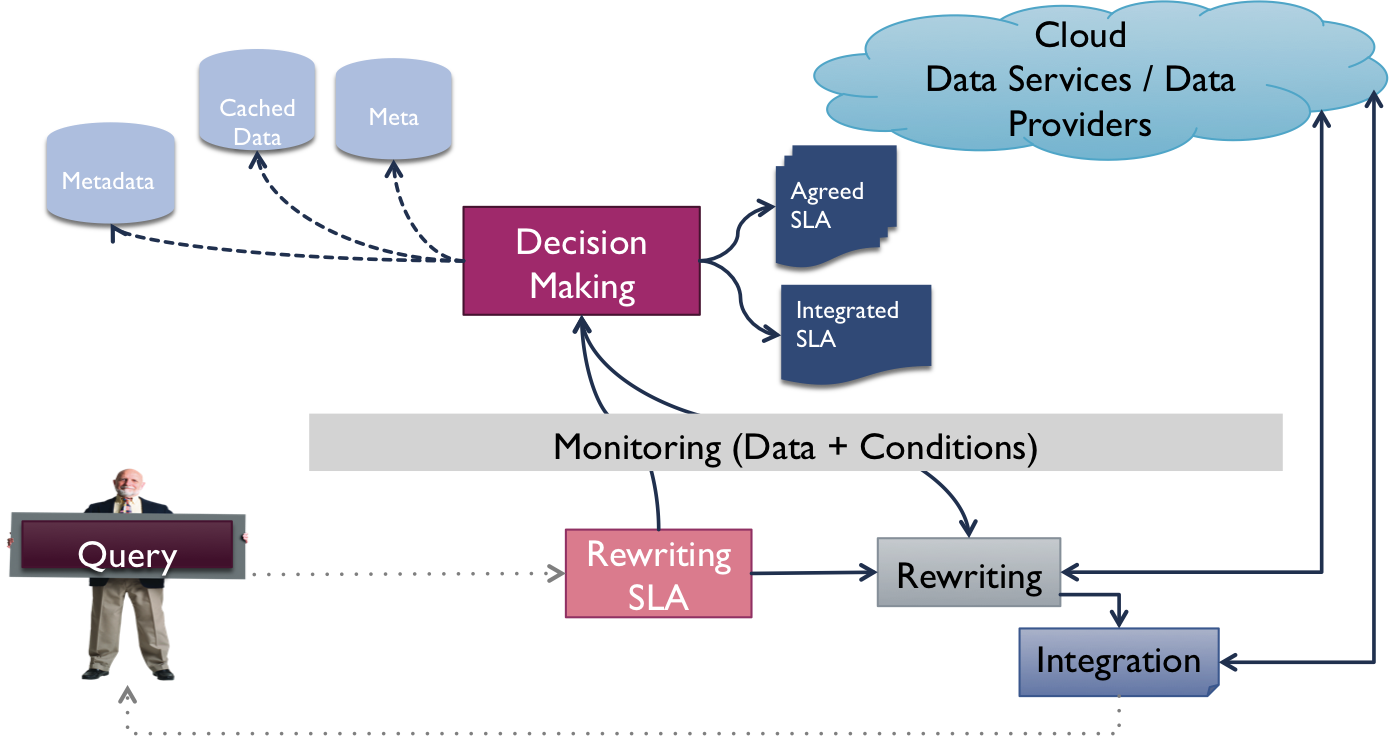
\includegraphics[width=0.8\textwidth]{figs/arch.png}
\caption{General architecture of an SLA guided  data integration system.\label{fig:arch}}
\end{figure*}

Figure~\ref{fig:arch} shows the general architecture of an SLA guided data integration system that is supported by data services which are data providers deployed in a cloud and that provide agreed SLA’s. 
These descriptions are stored in a directory together with meta-data about the way queries are evaluated for producing results. 
The system uses this information  by query processing and monitoring modules for rewriting queries according to given quality of service (QoS) preferences expressed by a data consumer, for example a user.


Consider a smart city that aims at being energy self-sustainable and produce and consume as much as possible, energy within its geographic area. 
Producers are characterized according to their location, the amount of energy in kWatts-hour that they can sell, the cost, and the time window in which they can produce it, with a given service level agreement concerning their availability and fault tolerance. 
Consumers, give also their location, their energy requirements during a certain interval of time, the maximum total cost they are ready to pay, and quality of service requirements such as availability and how critical it is to consume this amount of energy. 
A energy exchange market is established in order to continuously trade  energy provision/consumption ensuring that all consumers will have the energy they require at every moment.

\begin{figure*}
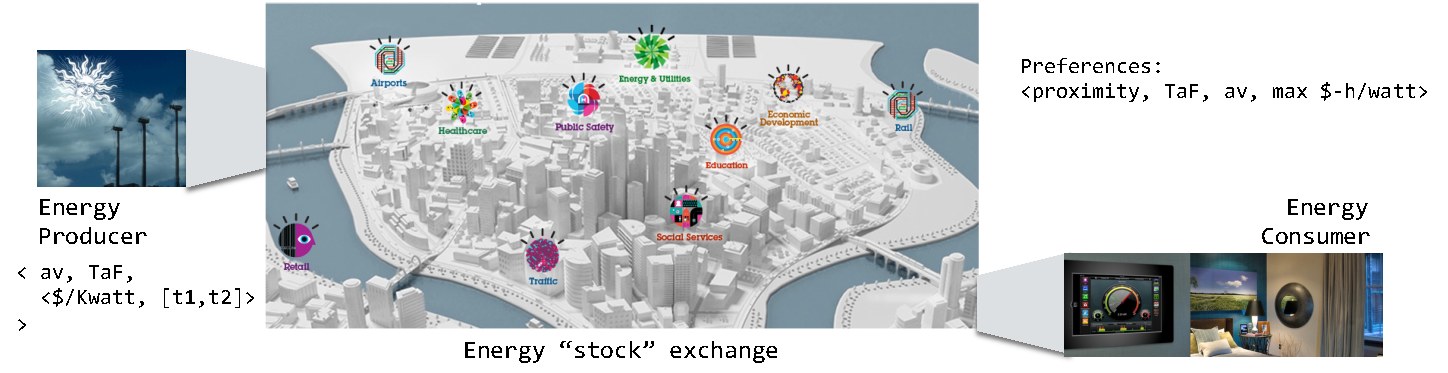
\includegraphics[width=0.95\textwidth]{figs/exchange.pdf}
\caption{\label{fig:energyXChange} Energy exchange.}
\end{figure*}

In our approach energy producers are modelled as services with associated ``agreed'' SLAs. 
In general, we assume that several producers will be able to supply energy for a given period of time given specific  preferences expressed by a consumer. 
An energy request is expressed as a query that specifies an energy requirement with QoS preferences independently of the possible producers. In our example assume that there are several energy provision services (e$_1$, ... e$_n$) that can be independent or hubs:
\begin{description}
\item energyProvider.requestAvailability() $\rangle$ $<$ KWatt/h, cost, rate, location $>$ $\langle$

\item energyHub.requestAvailability() $\rangle$ $<$ {ID, KWatt/h, cost, rate, location $>$}$\langle$
\end{description}

 Given a query, expressed as an SQL like expression including spatio-temporal attributes and preferences, for example, {\em List of energy providers that can provision 1000 Kwatts/h, in the next 10 seconds, that are close to my city with a cost of 0,50 euros/Kwatt?}. Assuming also that energy providers are represented by services exporting their SLA agreements and that can potentially be combined for answering the query. 


\section{\uppercase{Conclusions and Future work}}
\label{sec:conclusions}
This paper introduces the challenge of integrating data from distributed data services deployed on different cloud providers guided by service level agreements (SLA) and user preferences statements. The data integration problem is stated as a continuous data provision problem that has an associated economic cost and that uses automatic learning techniques for ensuring different qualities of delivered data (fresh, precise, partial).



Current big data settings impose  to consider SLA and different data delivery models. We believe that given the volume and the complexity of query evaluation that includes steps that imply greedy computations, it is important to combine and revisit well-known solutions  adapted to these contexts. We are  developing  strategies and algorithms overviewed in this paper and applying them to energy consumption applications and to elections and political campaign data integration to guide decision making on campaign strategies.

The diversity of mentioned application domains highlights the difficulty regarding SLA manipulation. Indeed, cloud, service, and user SLAs could be expressed differently in term of clauses, formalism and content. The multi-cloud environment emphasizes this heterogeneity. 

 
The main issue when launching an integration process is to obtain the most accurate answer meeting the best user preferences. One of the possibilities when studying the integration is to accept the integration process in an incremental  manner so that the query will continue to be evaluated till satisfying the set of QoS and non functional constraints expressed by the user. To our knowledge, the incremental production of a solution is beyond  the scope of the current methods for rewriting service compositions and represents a challenge to the area.
Furthermore, the integration SLA generation step is outstanding study. In fact the integration SLA should indicate the negotiation result with the aim to reuse it in further integration.


% 
%\begin{example}[Incremental queries]\label{Ex:rew2}
%Let us return to the content  trade system of the MOOC example.
% Suppose that the user requires to retrieve a list of star providers  daily and weekly that can deliver ``\textit{5 Go}'' of expert content about Emily Dickinson poetry.
%In this case, each individual and hub database will be queried and the list will be produced by adding data obtained from them, until the 5Go  capacity is reached.
%Let us suppose that, in order to minimize the  communications between servers, the lists need to be produced incrementally.
%In this case, the composition produced by the service refinement may need to include an iteration (to aggregate partial results). 
%The data produced by the warehouse servers will be processed in batch and the process will end once the list reaches the desired capacity.
%
%
%~\hfill\openbox
%\end{example}
%
%\color{black}




%\vfill
\bibliographystyle{apalike}
{\small
\bibliography{example}}


%\section*{\uppercase{Appendix}}


%\vfill
\end{document}

